\chapter{Simulation of Atmospheric Conditions over First-Year Sea Ice using the Polar Weather Research and Forecasting Model}
\vspace{1 cm}
\begin{spacing}{1} \begin{quote} 
\noindent \emph{The polar regions, notably the Arctic and maritime Antarctic, are experiencing impacts from climate change at magnitudes and rates that are among the highest in the world, and will become profoundly different in the near-term future (by 2050) under all warming scenarios (high confidence).}\end{quote}
\hspace{6 cm} - IPCC Sixth Assessment Report, August 2021  
\end{spacing}
\doublespacing
\section{Introduction}
The Arctic has experienced large changes and dramatic loss in sea ice throughout the twenty-first century \citep{hines:2015}, signifying a transition in the Arctic from primarily thick, multi-year ice to thin, first-year sea ice. Increases in thin, first-year sea ice and open water have resulted in climate modeling errors not only in the polar regions but elsewhere on Earth \citep{hines:2015, royer:1990, francis:2009}. 

The Polar Meteorology Group at the Ohio State University Byrd Polar Research Center developed a series of enhancements to the Weather Research and Forecasting Model (WRF). These modifications include enhanced mechanisms to allow prescribed sea ice thickness (default in non-polar WRF is 3 $m$), as well as sea ice fraction and snow depth \citep{hines:2015}. These mechanisms are primarily implemented as sea ice enhancements in the land surface model (Noah LSM), but also include the heat transfer and thermal diffusivity through the snow and ice. albedo, snow density adjustments, and skin temperature calculations \citep{tastula:2012, hines:2015}. This model was developed as the successor to the Polar fifth-generation Mesoscale Model (MM5) with advanced physical parameterizations \citep{bromwich:2009}. It has been used extensively for weather forecasting in Antarctica \citep{powers:2012} and has been tested over ice and land in the Arctic \citep{tastula:2012, bromwich:2009}. 

In spite of Polar WRF being available for over 10 years, the model has only undergone limited testing in the Arctic with no testing over young thin sea ice. This chapter uses the data collected from a comprehensive suite of instruments deployed during the Norwegian Young Sea Ice field campaign in 2015 (N-ICE) to test and evaluate the performance of Polar WRF over young thin sea ice. 

\section{Observations and Model Setup}
In this modeling study, observations from the N-ICE were used to evaluate the Polar WRF model. The model was run for a 6-month period (1 January 2015 to 1 July 2015) for selected combinations of planetary boundary layer (PBL) and cloud microphysics (CM) schemes; this time period overlapped with the entire N-ICE campaign. Three case study periods were selected for further analysis using idealized model runs using radiosonde soundings taken during N-ICE as input.

\subsection{Observations}
Details about the N-ICE field campaign can be found in Chapter 2. Most notable for the analysis presented here are the atmospheric radiation measurements, taken by Kipp and Zonen (CMP22 and CGR4) radiometers mounted 1 to 1.2 $m$ above the ground. \citet{granskog:2015} and \citet{walden:2017} include a complete analysis of the radiative fluxes during N-ICE, which includes a description of how surface temperatures were calculated. \citet{walden:2017} also showed that the radiative fluxes during N-ICE were primarily influenced by wind, advection, and cloud cover. 

\subsection{Model Setup}

The WRF model version 4.1.4 was run with polar optimizations created by researchers at The Ohio State University. WRF with polar optimizations is often referred to as Polar WRF. WRF is a mesoscale weather model developed with both numerical weather prediction and research applications in mind. It is maintained by the NCAR's Mesoscale and Microscale Meteorology Laboratory (MMM). As of 2021, WRF had over 57,800 registered users. The model allows users to select many options, such as domain size, temporal and spatial resolution, and input datasets \citep{skamarock:2019}.

\begin{figure}[h]
    \centering
    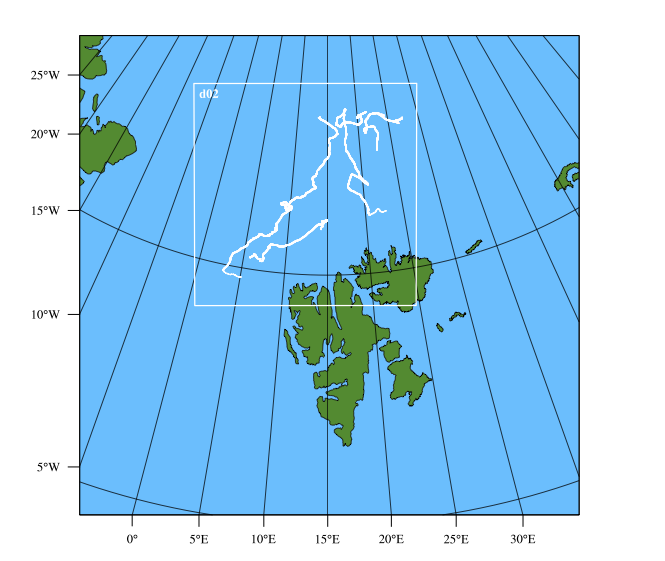
\includegraphics[width=1\linewidth]{figures/chapter3/wrf_domain.png}
    \caption[WRF Model Domain]{The WRF model domain (parent) with N-ICE domain (d02) in a 2-way nested configuration. The N-ICE ship tracks are in white.}
    \label{fig:wrf_domain}
\end{figure}

A 2-way nested, two-domain (parent and nested domain) setup was used and can be seen in Figure \ref{fig:wrf_domain}. The nested domain (d02) used 3 $km$ by 3 $km$ grid cells, located just north of Svalbard and encompassing the entire spatial extent of the N-ICE field campaign. The larger domain, or the parent domain, used 9 $km$ by 9 $km$ grid cells. The European Centre for Medium-Range Weather Forecasting’s Interim Re-Analysis (ERA-Interim) was used for boundary and initial conditions \citep{dee:2011}, Pan-Arctic Ice Ocean Modeling and Assimilation System (PIOMAS) was used for snow depth, ice thickness, and albedo \citep{PIOMASS}, and Special Sensor Microwave/Imager (SSMI) was input for ice extent information \citep{SSMI, schweiger:2011}. \citet{graham:2017} includes a comparison of the ERA-Interim dataset and the measurements taken during N-ICE. While \citet{graham:2017} found that ERA-Interim accurately portrayed the cloudy and clear states, there were still issues with the cloud liquid water path being underestimated, which should be taken into consideration when looking at the WRF results. The model was run for two periods: winter (January through March) and spring (April through June). Comparison with the N-ICE measurements for these periods start on 15 January and 18 April, resulting in 15+ days of spin-up time of the Polar WRF model before analysis. The simulations were completed using the Cheyenne supercomputer \citep{cheyenne}. More details about model settings are shown in Table \ref{tab:setup}. 

\begin{table}[t]
\centering
\footnotesize
\doublespacing
{
\begin{tabular}{| c | c |}
\hline
\rowcolor[HTML]{F3F3F3} \multicolumn{2}{|c|}{\textbf{Dates}} \\
\hline
Winter & 1 January - 1 April 2015 \\
Spring & 1 April - 1 July 2015 \\
\hline
 \rowcolor[HTML]{F3F3F3} \multicolumn{2}{|c|}{\textbf{Input Datasets}} \\
\hline
 Boundary and initial conditions & ERA-Interim \\
 Snow depth, ice thickness, and ice extent & PIOMASS and SSMI \\
\hline
\rowcolor[HTML]{F3F3F3} \multicolumn{2}{|c|}{\textbf{Polar WRF Settings}} \\
\hline
 LW and SW Radiation Scheme & RRTMG \\ 
 Surface Layer Scheme & Revised MM5 or ETA Similarity \\
 Land Surface & Unified Noah Land Surface Model  \\ 
  \hline
\end{tabular}}
\caption[WRF input datasets, dates, and settings.]{Input datasets and settings used for all Polar WRF simulations. ETA Similarity surface layer scheme was only used in cases with the MYJ PBL scheme.}
\label{tab:setup}
\end{table}

In addition to the choice of input datasets and the underlying models used, one can select from a variety of different schemes to control different physical processes in the atmosphere and at the surface. This study focuses on the evaluation of different PBL and CM schemes because of their importance to Arctic conditions. The schemes used here were selected after a thorough literature review of previous WRF studies of both polar and non-polar applications. Various PBL schemes were selected to determine which of them most accurately represents the strong near-surface inversion in the Arctic. Clouds also have strong radiative importance in the Arctic, so a variety of CM schemes were selected to determine which provide accurate representations of Arctic clouds, including the presence of mixed-phase (water and ice) and supercooled water clouds. All other schemes, with the exception of the surface layer scheme, were kept constant throughout all simulations. Table \ref{tab:schemes} shows all PBL and CM schemes chosen for this study and the abbreviations used to refer to each model run. 

\begin{figure}[p!]
    \centering 
    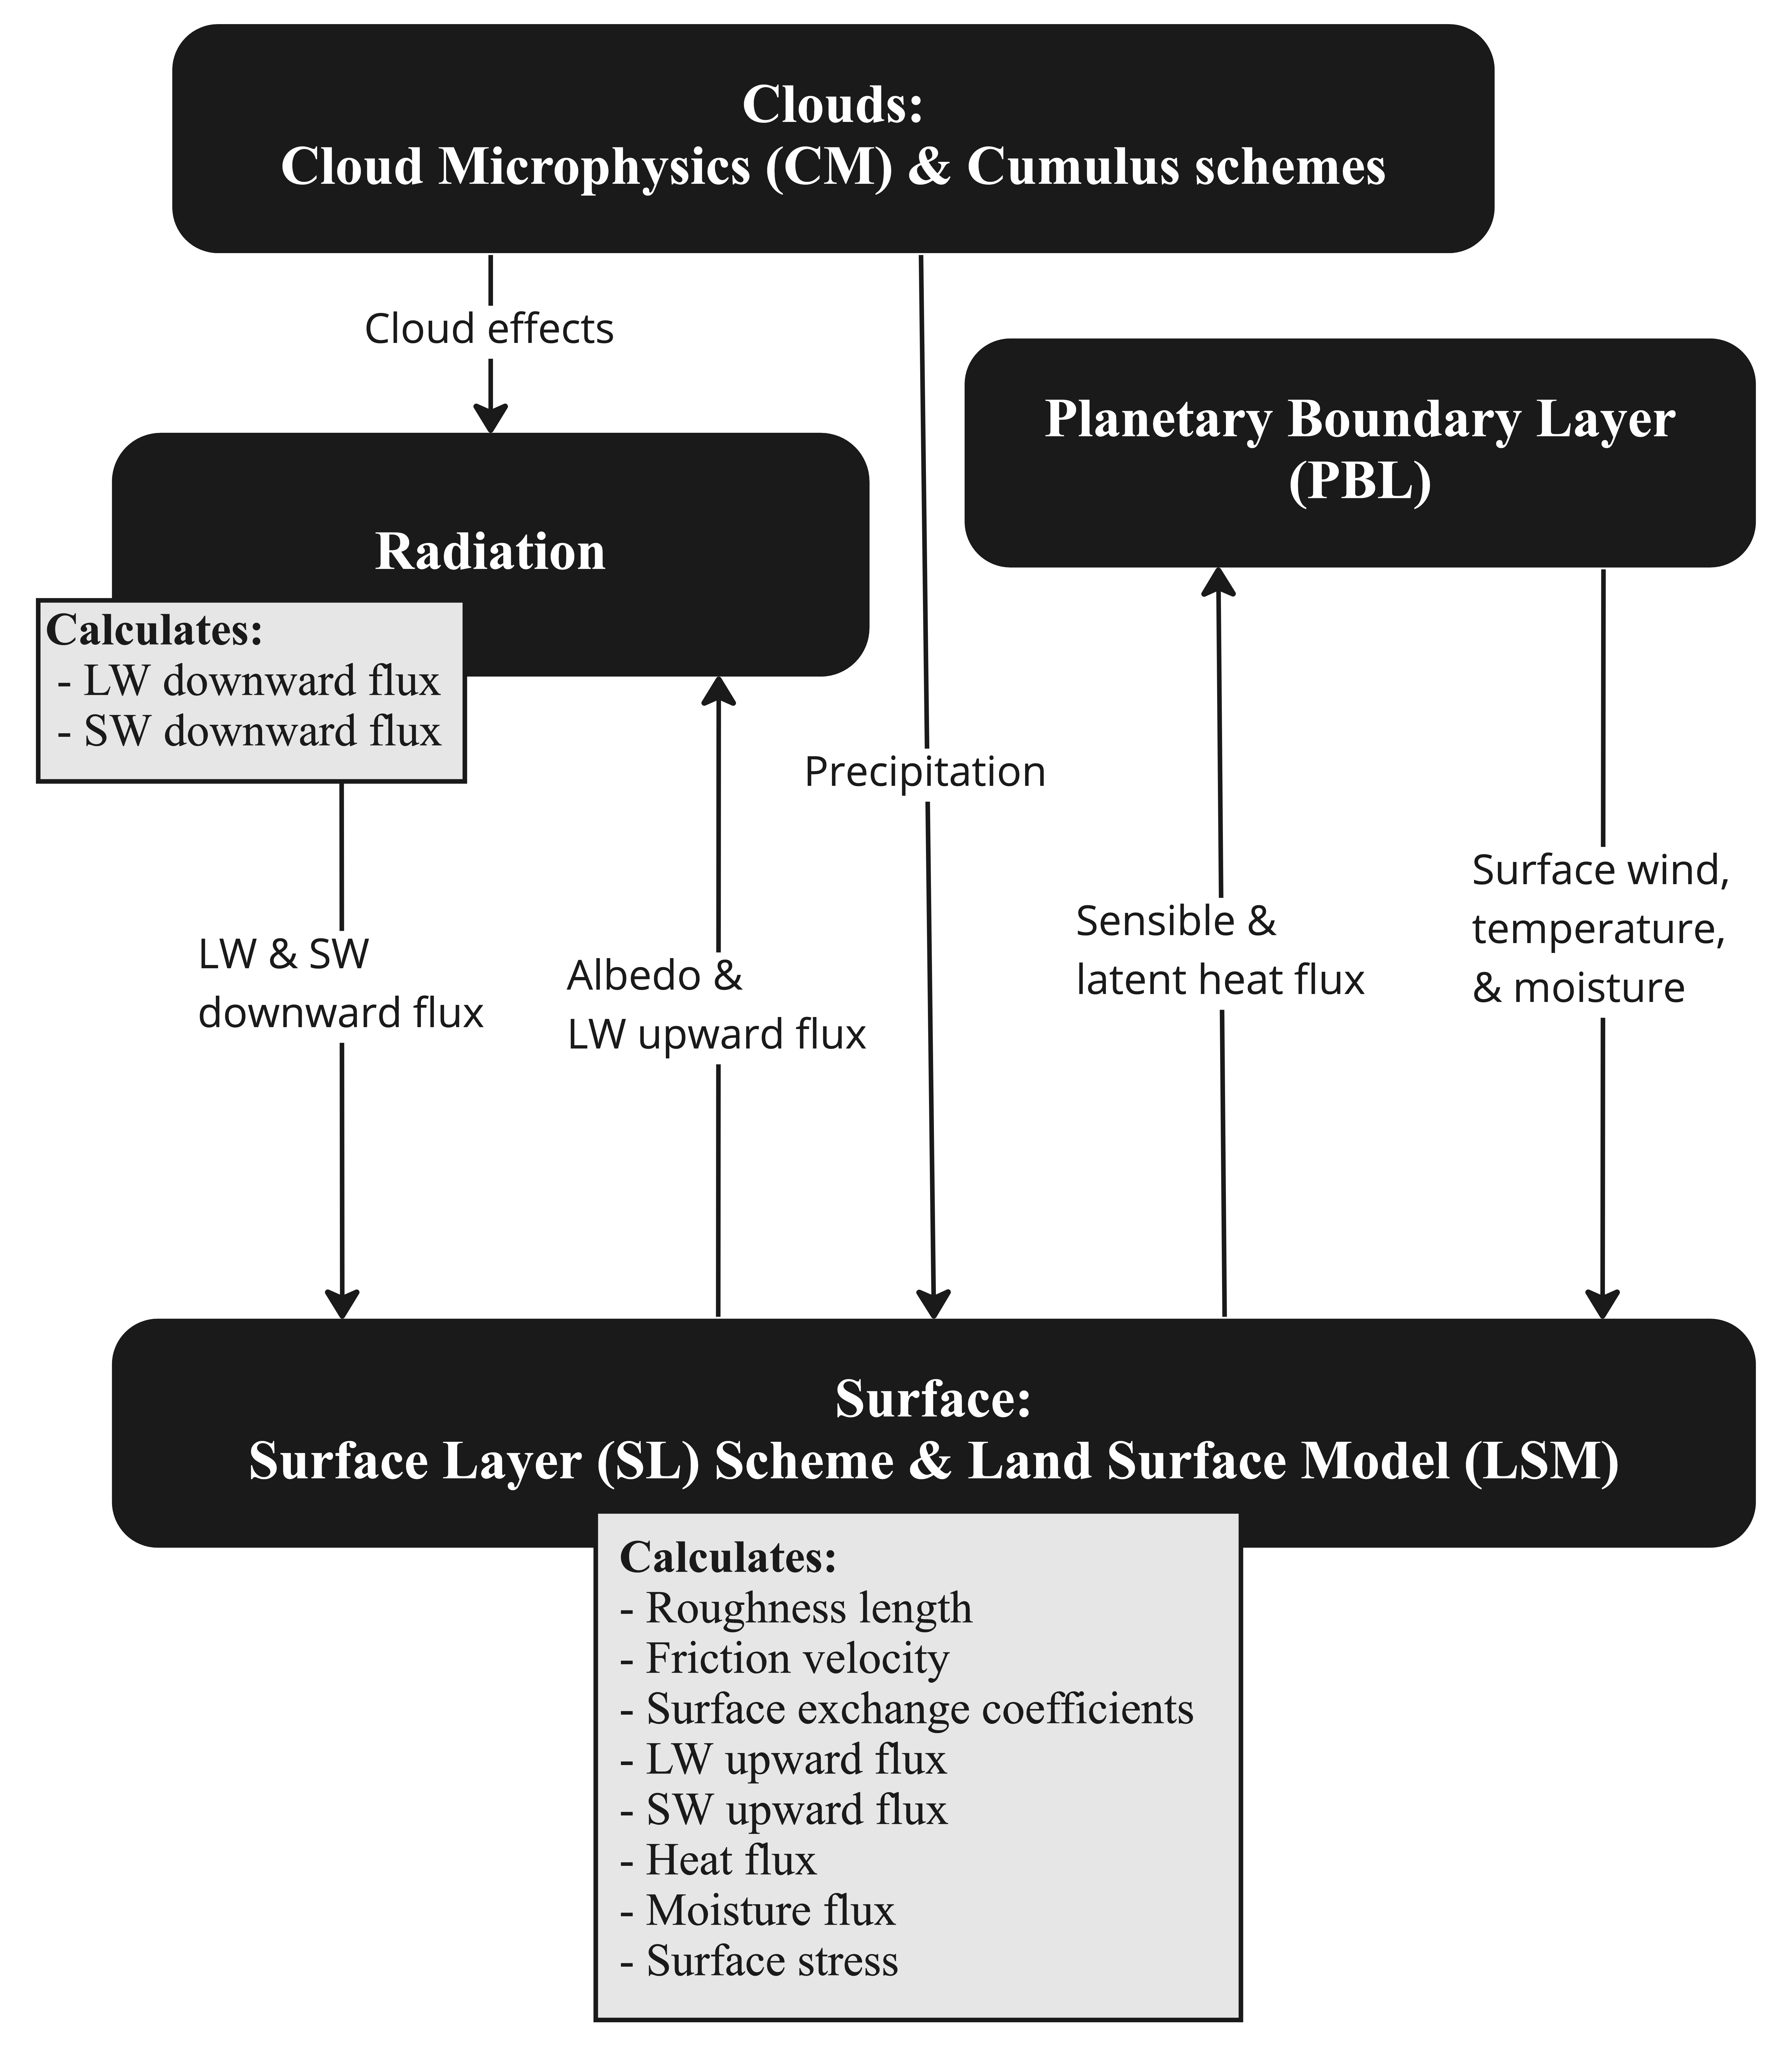
\includegraphics[width=1\linewidth]{figures/chapter3/WRF_Flowchart.jpg}
    \caption[WRF Model physics scheme exchanges.]{The relevant WRF model physics schemes, variables exchanges, and calculations used in this study.}
    \label{fig:wrfflow}
\end{figure}

In addition to the PBL and CM schemes, a radiation scheme, surface layer scheme, and land surface model (LSM) must be selected. Unified Noah Land Surface Model (Noah LSM) was selected as the LSM. The Noah LSM has been tested and improved over polar regions, and its tuning is a key strength of Polar WRF \citep{mukul:2004, hines:2015, tewari:2004}. Further exploration of the Noah LSM can be found in Chapter 6. The Rapid Radiative Transfer Model (RRTMG) was selected to handle longwave and shortwave radiation \citep{mlawer:1997} and the Revised MM5 surface layer scheme was used for all model simulations except those with the Mellor–Yamada–Janjic (MYJ) PBL scheme \citep{jimenez:2012}. The ETA Similarity surface layer scheme is required by the model to use the MYJ PBL scheme \citep{janic:2001}. Figure \ref{fig:wrfflow} is a flowchart showing the key physics schemes, variable exchanges, and relevant calculations in the model.

\begin{table}[t]
\doublespacing
\centering
\footnotesize
{\begin{tabular}{| c | c | c | c | c | c |}
  \hline
 \rowcolor[HTML]{F3F3F3} & & \multicolumn{4}{c|}{\textbf{CM Schemes}} \\
 \rowcolor[HTML]{F3F3F3} & & \textbf{Goddard} & \textbf{WRF 5-Class} & \textbf{Predicted Particle} & \textbf{Morrison 2-Moment} \\
  \hline
\cellcolor[HTML]{F3F3F3}
 &\textbf{YSU} & G-YSU & & P3-YSU & \\
\cellcolor[HTML]{F3F3F3}  & \textbf{MYJ} & G-MYJ & 5-MYJ & P3-MYJ & 2-MYJ \\ 
\cellcolor[HTML]{F3F3F3}  \parbox[t]{3mm}{\multirow{-3}{*}{\rotatebox[origin=c]{90}{\textbf{PBL}}}} \parbox[t]{2mm}{\multirow{-3}{*}{\rotatebox[origin=c]{90}{\textbf{Schemes}}}} & \textbf{MYNN} & G-MYNN & 5-MYNN & & 2-MYNN \\
  \hline
\end{tabular}}
\caption[Cloud microphysics and planetary boundary layer schemes used in polar WRF simulations.]{Cloud microphysical (CM) and planetary boundary layer (PBL) schemes used for Polar WRF model simulations with corresponding abbreviations used to refer to each model run.}
\label{tab:schemes}
\end{table}

% Planetary boundary layer schemes
The most commonly used PBL schemes found in the literature were the Yonsei University (YSU) scheme \citep{hong:2004} and MYJ scheme. The Mellor–Yamada Nakanishi Niino (MYNN) scheme \citep{olson:2019} is a modified version of the MYJ scheme \citep{mesinger:1993}. The MYNN scheme has been tested over Svalbard, a location close to the N-ICE domain but with different surface conditions \citep{pilguj:2018}. Development of the MYNN scheme focused on large eddy diffusion \citep{cohen:2015}, while the MYJ scheme is focused more on stable flows \citep{janjic:1994, mellor:1982}. MYJ is a 1.5-order closure scheme and MYNN is a 2nd-order closure scheme \citep{pilguj:2018}. Higher order closure indicates that fewer assumptions are made in calculating turbulence. Closure in modeling turbulent fluxes is an issue that arises in Monin-Obukhov similarity theory due to need for estimations in the equations to calculate the fluxes. A higher-order closure will give more accurate results at a higher computational expense. 

% Cloud microphysical schemes
The Goddard (G) scheme \citep{tao:2000} and WRF Single-Moment 5-Class (5) scheme \citep{hong:2004} are the two most commonly used CM schemes found from the literature search regardless of the location being modeled. The Predicted Particle Properties (P3) scheme is a newly released scheme with advancements to the Morrison Two-Moment (2) scheme \citep{milbrandt:2016, morrison:2015}. This scheme was not designed for the polar regions but is of particular interest due to the way it parameterizes ice particle density. Many CM schemes use bins to classify different cold cloud particle sizes and densities, leading to assumptions that can potentially lead to large errors. The P3 scheme eliminates the conversion between categories by using one set of parameters that evolve throughout the lifecycle of the cloud particles. This reduces the simplifications often made when using the binning approach for ice particles \citep{morrison:2005}. However, this scheme has a particle size cutoff, eliminating smaller particles, which may prove to be problematic in the dry polar regions.

\begin{figure}[p!]
    \centering
        \vspace*{-1cm}
    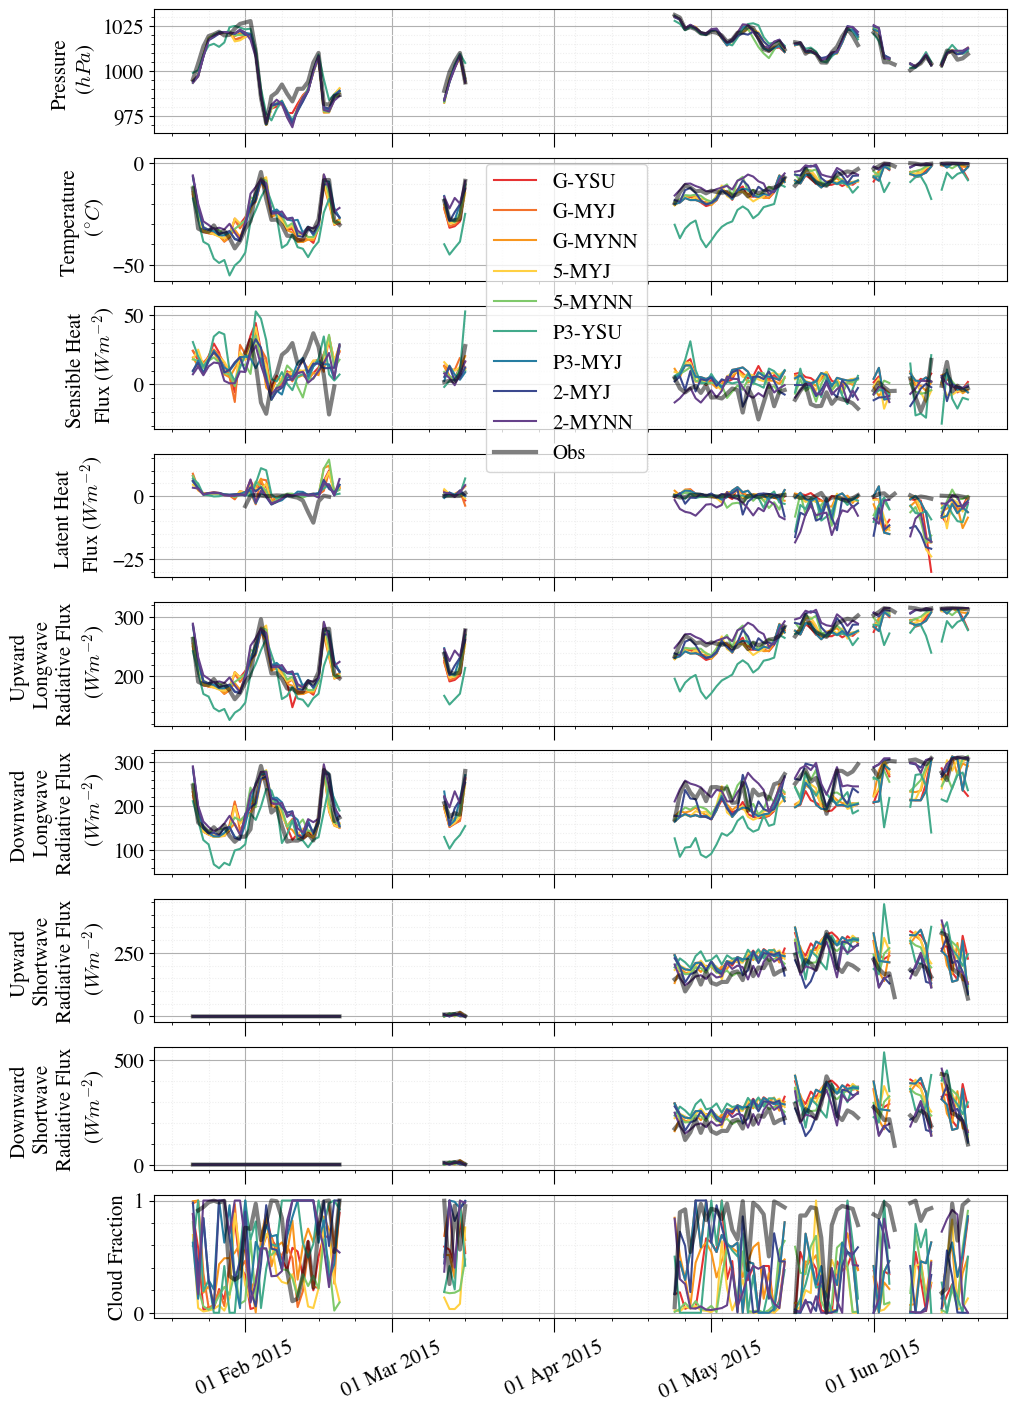
\includegraphics[width=1\linewidth]{figures/chapter3/WRF_totaltimeseries.png}
    \caption[Polar WRF simulated temperature, pressure, sensible and latent heat flux, components of longwave and shortwave flux, and cloud fraction time series.]{Daily averages of temperature (top), sensible heat flux (second from top), latent heat flux (third), upward and downward longwave flux (fourth and fifth), upward and downward shortwave flux (sixth and seventh), and cloud fraction (bottom). Measurements are shown in black and each model simulation is a different color, identified by the abbreviations defined in Table \ref{tab:schemes}.}
    \label{fig:wrf_all}
\end{figure}

\section{Results}
Atmospheric conditions at the grid cell containing the ship were selected from the model output. Time series of the temperature, sensible and latent heat fluxes, components of longwave and shortwave flux, and cloud fraction in the model grid cell at the ship location can be seen in Figure \ref{fig:wrf_all}. While it is difficult to see fine details in these panels, the P3-YSU scheme stands out during both the winter and spring, with particularly low values of temperature, upward longwave flux, and downward longwave flux. Additionally, cloud fraction values are greatly varied between model runs, and are often not in agreement with the observations. Further analysis of each variable is included in the following subsections.

Eq. \ref{eq:modbias} was used to calculate mean model biases from the time series for skin temperature ($K$), latent heat flux ($Wm^{-2}$), sensible heat flux ($Wm^{-2}$), net longwave flux ($Q_{sw}$, $Wm^{-2}$, Eq. \ref{eq:netlwflux}), and net shortwave flux ($Q_{sw}$, $Wm^{-2}$, Eq. \ref{eq:netswflux}) and are shown in Table \ref{tab:meanbias} for winter (top) and spring (bottom). In this equation, $y_{mod}$ is the modeled value and $y_{obs}$ is the observed value.
 
\begin{equation}\label{eq:modbias}
Mean~bias = \frac{1}{n}\sum^{n}_{i=1}(y_{mod} - y_{obs})
\end{equation}

\begin{equation}\label{eq:netlwflux}
Q_{lw} = Q_{lw \downarrow} - Q_{lw \uparrow}
\end{equation}

\begin{equation}\label{eq:netswflux}
Q_{sw} = Q_{sw \downarrow} - Q_{sw \uparrow}
\end{equation}

 Bias values were only calculated for times when measurements were available. Negative (positive) model biases indicate the model is producing values lower (higher) than those observed. The mean bias was selected as a way to determine model accuracy as it allows for a quick summary of how much the modeled time series disagrees with the measured values, although it can hide compensating biases at different times or under different conditions. The primary goal of this study is to determine which schemes perform well and which combinations of schemes give unreasonable values. A complete table with mean bias, correlation, and root mean square error is included in Table \ref{tab:wrfstats} in Appendix C. 

\begin{table*}[p]
\center
\centering
\footnotesize
\doublespacing
{
\begin{tabular}{| l | c | c | c | c | c |}
\hline
\rowcolor[HTML]{F3F3F3} & \multicolumn{5}{ c|}{\textbf{Winter}} \\
\rowcolor[HTML]{F3F3F3} & \textbf{Temperature} & \textbf{Latent Heat} & \textbf{Sensible Heat} & \textbf{Net LW} & \textbf{Net SW} \\
\hline
\rowcolor[HTML]{F0F8E6}\textbf{G-YSU} & 0.3 & -1.0 & -23.4 & 2.9 &  \\
\rowcolor[HTML]{E0EDF4}\textbf{G-MYJ} & -0.1 & -0.3 & -22.6 & 4.4 & \\
\rowcolor[HTML]{FEEEF5}\textbf{G-MYNN} & 0.2 & -1.3 & -21.0 & 5.1 & \\
\rowcolor[HTML]{E0EDF4}\textbf{5-MYJ} & 0.7 & -0.8 & -23.0 & 3.4 & \\
\rowcolor[HTML]{FEEEF5}\textbf{5-MYNN} & 2.0 & -1.2 & -18.5 & 8.5 & \\
\rowcolor[HTML]{F0F8E6}\textbf{P3-YSU} & -7.5 & -1.1 & -25.0 & -2.5 & \\
\rowcolor[HTML]{E0EDF4}\textbf{P3-MYJ} & 3.1 & 0.4 & -17.2 & 12.9 & \\
\rowcolor[HTML]{E0EDF4}\textbf{2-MYJ} & 2.2 & -0.1 & -18.3 & 10.2 & \\
\rowcolor[HTML]{FEEEF5}\textbf{2-MYNN} & 4.5 & 0.1 & -17.1 & 12.0 & \\
\hline
\rowcolor[HTML]{F3F3F3} & \multicolumn{5}{c|}{\textbf{Spring}} \\
\rowcolor[HTML]{F3F3F3} & \textbf{Temperature} & \textbf{Latent Heat} & \textbf{Sensible Heat} & \textbf{Net LW} & \textbf{Net SW} \\
\hline
\rowcolor[HTML]{F0F8E6}\textbf{G-YSU} & -2.6 & 2.3 & 2.2 & -33.0 & 2.2 \\
\rowcolor[HTML]{E0EDF4}\textbf{G-MYJ} & -2.4 & 2.0 & 2.0 & -32.0 & 2.0 \\
\rowcolor[HTML]{FEEEF5}\textbf{G-MYNN} & -1.8 & 2.7 & 4.1 & -27.1 & 4.1 \\
\rowcolor[HTML]{E0EDF4}\textbf{5-MYJ} & -2.0 & 2.7 & 4.0 & -29.2 & 4.0 \\
\rowcolor[HTML]{FEEEF5}\textbf{5-MYNN} & -0.7 & 3.3 & 6.3 & -22.0 & 6.3 \\
\rowcolor[HTML]{F0F8E6}\textbf{P3-YSU} & -9.4 & 3.3 & 6.1 & -32.2 & 6.1 \\
\rowcolor[HTML]{E0EDF4}\textbf{P3-MYJ} & -2.4 & 2.0 & 2.0 & -32.1 & 2.0 \\
\rowcolor[HTML]{E0EDF4}\textbf{2-MYJ} & -0.1 & 4.9 & 7.5 & -13.7 & 7.5 \\ 
\rowcolor[HTML]{FEEEF5}\textbf{2-MYNN} & 2.2 & 6.5 & 10.3 & -3.3 & 10.3\\
\hline
\end{tabular}
\caption[Polar WRF mean model bias for temperature, latent heat flux, sensible heat flux, net longwave flux, and net shortwave flux.]{Mean model bias for temperature ($K$), latent heat flux ($Wm^{-2}$), sensible heat flux ($Wm^{-2}$), net longwave flux (Net LW) ($Wm^{-2}$), and net shortwave flux (Net SW) ($Wm^{-2}$). Acronyms in the left-hand column represent the CM and PBL schemes and are defined in Table \ref{tab:schemes}. Rows are ordered by CM scheme and colored by PBL scheme for ease of use.}
\label{tab:meanbias}
\end{table*}}

\subsection{Skin Temperature}
G-MYJ had the smallest mean temperature bias in winter. For spring, 2-MYJ had the smallest model bias. Figure \ref{fig:wrf_tsk} shows the distribution of skin temperature from each model run with the measurements shown in black. P3-YSU has colder temperatures than the measurements and all model runs throughout the entire experiment and, as a result, has the largest biases in skin temperature in both seasons. 

\begin{figure}[b!]
    \centering
    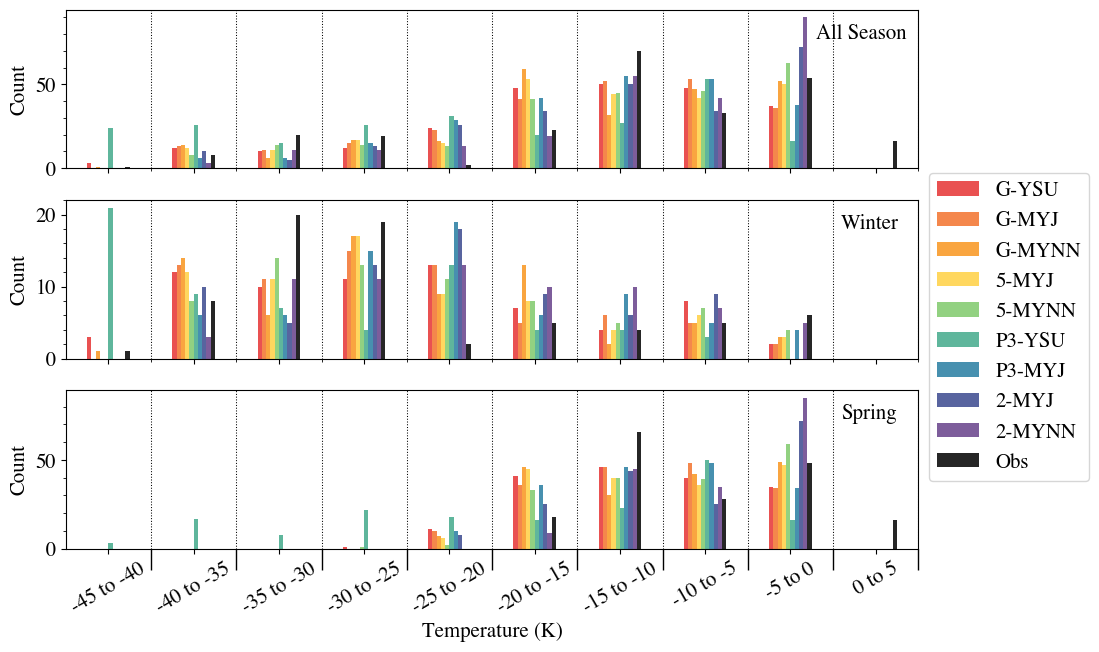
\includegraphics[width=1\linewidth]{figures/chapter3/WRF_TSK_Histo.png}
    \caption[Polar WRF simulated temperature histograms.]{Temperature for the entire observational period (top), winter (middle), and spring (bottom) for each of the Polar WRF runs. Measurements are shown in black and each model simulation is a different color, identified by the abbreviations defined in Table \ref{tab:schemes}.}
    \label{fig:wrf_tsk}
\end{figure}

Some of these disagreements between the model and measurements can be attributed to inaccurate surface albedo and a lack of cloudiness. The model simulated the surface albedo to be around 0.2 less than the measured surface albedo (0.6 compared to 0.8 measured at N-ICE). The model surface temperature reaches the freezing point earlier than the observations. The transition season is when the model had the most difficulty in simulating the skin temperature, but in the summer, when the temperature reaches freezing, all of the model simulations agree well with the observations. 

\subsection{Longwave and Shortwave Fluxes}
In the winter, P3-YSU had the lowest bias in longwave flux. All other model simulations produced a positive bias in the winter. This suggests that the low bias in longwave flux is likely due to the strong negative temperature bias compensating for the overestimation of longwave flux occurring within the model. 

  \begin{figure}[t]
    \centering
    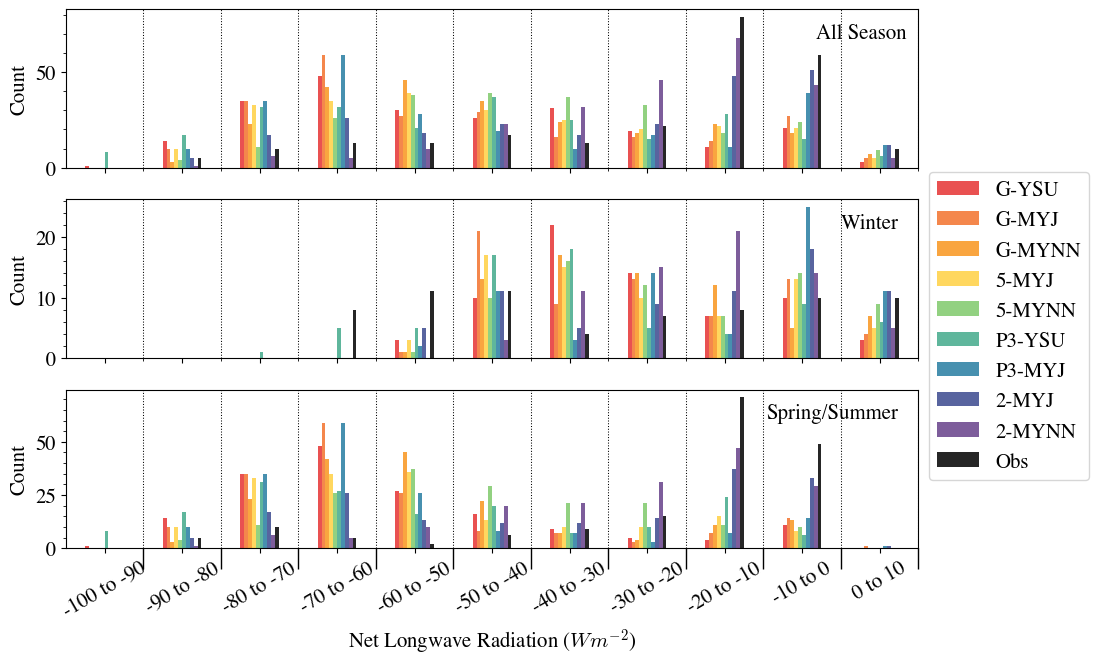
\includegraphics[width=1\linewidth]{figures/chapter3/WRF_NetLW_Histo.png}
    \caption[Polar WRF simulated net longwave flux histograms.]{Net longwave flux at the surface for the entire observational period (top), winter (middle), and spring (bottom) for each of the Polar WRF runs. Measurements are shown in black and each model simulation is a different color, identified by the abbreviations defined in Table \ref{tab:schemes}.}
    \label{fig:wrf_netlw}
\end{figure}

 In winter, the distributions shown in Figure \ref{fig:wrf_netlw} show two peaks in the observations (black bars). One peak shows a maximum between -60 and -40 $Wm^{-2}$ and corresponds to clear sky conditions. These conditions are most accurately modeled by G-YSU. This is further corroborated by the low biases seen in Table \ref{tab:meanbias} and Table C.1 in Appendix C. A second peak occurs around -10 $Wm^{-2}$ and is related to cloudy conditions, which is most accurately captured by 5-MYJ. Overall, the lowest net longwave biases were seen with the G-YSU and P3-YSU simulations, indicating that the YSU boundary layer scheme is producing the best surface-layer temperature structure during the winter at N-ICE. 
 
 Spring and summer longwave flux values were more largely negative in all model runs compared to the measurements. This indicates that the surface was losing more longwave flux than it was gaining, which is likely due to clouds in the models being either too cold or thin to produce the downward longwave flux required to balance out the amount of longwave being lost from the surface. In the spring, the downward longwave is clearly dominated by the CM schemes, as the schemes show vastly different results. The WRF 2-Moment CM scheme has the lowest net longwave biases in the spring by almost 20 $Wm^{-2}$ in some cases (Table \ref{tab:meanbias}). The 2-MYNN scheme has the lowest mean net longwave bias for spring, which indicates that this scheme may be producing clouds closest to what was actually observed. While the 2-MYNN does well with the spring and summer net longwave flux, this simulation had the largest biases in the net shortwave flux, which indicates that there may be some compensating errors in the turbulent fluxes.

\begin{figure}[h!]
    \centering
    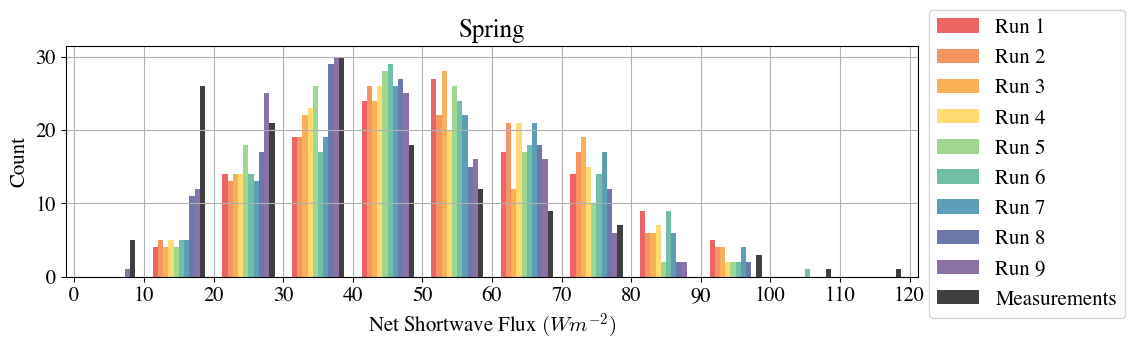
\includegraphics[width=1\linewidth]{figures/chapter3/WRF_NetSW_Histo.png}
    \caption[Polar WRF simulated net shortwave flux histograms.]{Net shortwave flux at the surface for the entire observational period (top), winter (middle), and spring (bottom) for each of the Polar WRF runs. Measurements are shown in black and each model simulation is a different color, identified by the abbreviations defined in Table \ref{tab:schemes}.}
    \label{fig:wrf_netsw}
\end{figure}

Net shortwave flux (Figure \ref{fig:wrf_netsw}) is only shown and calculated for spring and summer. The N-ICE location experienced 24-hour darkness in the winter until the sun rose in early March, at which time the hours of daylight increased until late April, when the field site experienced 24 hours of sunlight \citep{walden:2017}. The net shortwave flux is slightly larger in the model runs than in the measurements. The distributions from the model runs peak between 40 and 60 $Wm^{-2}$. These values are 10 to 20 $Wm^{-2}$ higher than the measurements, with the peak of the distributions correlating with the CM scheme used. 

The observations display two peaks. A second peak, which is not well replicated in the model distributions, can be seen in the measurements between 10 and 20 $Wm^{-2}$. This is likely a result of the low modeled albedo. The low sun angle, in combination with high early spring albedo, could result in these low net SW values. Shortwave flux was best represented in the G-MYJ and P3-MYJ schemes. These simulations also had the largest net longwave biases, so errors in the shortwave (and the sensible and latent heat fluxes) are compensating for the earth's radiation balance and are attempting to compensate for errors in other variables. Additionally, upward shortwave flux was hindered by an unreasonably low surface albedo in all model simulations.

\begin{figure}[h!]
    \centering \hspace*{-0.5cm}
    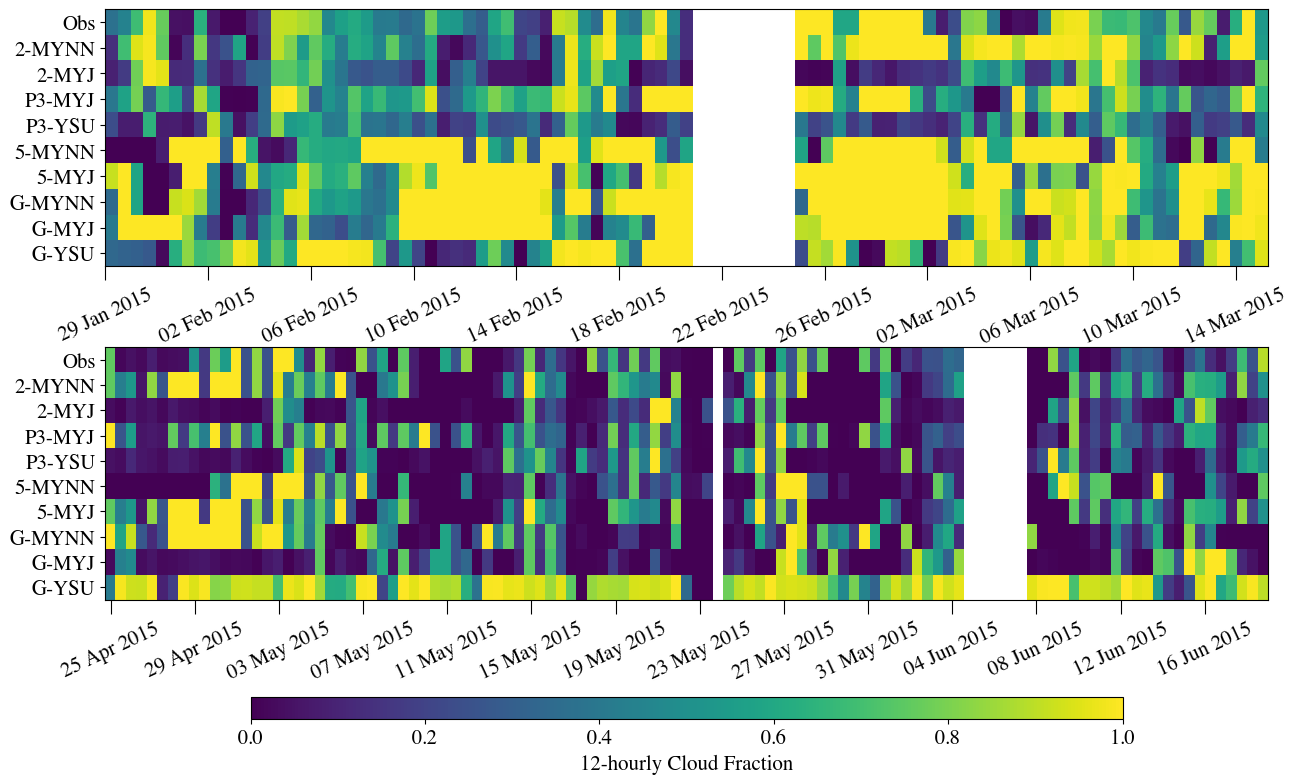
\includegraphics[width=1.1\linewidth]{figures/chapter3/WRF_Clouds.png}
    \caption[Polar WRF simulated cloud fraction.]{Cloud fraction from each Polar WRF run and the measurements in winter (top) and spring (bottom). Cloud cover is indicated by color, with yellows representing more cloud cover and purples less. Dark purple represents no cloud cover. Areas of white indicate no measurements. Polar WRF simulations are indicated on the left side of the figure by acronyms defined in Table \ref{tab:schemes} and observations represent was what actually observed at N-ICE.}
\label{fig:wrf_cloudfrac}
\end{figure}

Cloud cover was consistently present, particularly in spring and summer. However, the radiative fluxes in the model show that either the cloud fraction was not large enough or the clouds were not optically thick enough in any of the simulations. Figure \ref{fig:wrf_cloudfrac} shows the 12-hourly average cloud fraction in the grid cell corresponding to the ship location for each model run. The row labeled ``Obs" (bottom) on each panel is a 12-hourly vertical cloud fraction. This represents the frequency of occurrence of clouds in the entire column. While these are different metrics of calculating cloud fraction, they can give valuable insight into what the cloud cover was each day. For example, in the spring, at least 75$\%$ cloud cover was present almost the entire time with only one day (23 May 2015) classified as ``clear sky." This day can be seen by a blue stripe in Figure \ref{fig:wrf_cloudfrac}. Figure \ref{fig:wrf_cloudfrac} also shows that the cloud cover was less consistent in winter. 

One period of extended clear sky in the winter (9 February to 12 February) was captured best by model runs using the Goddard and WRF Single-Moment 5-Class CM schemes, with little apparent correlation to PBL scheme. The third major storm period at N-ICE (M3, 15 February to 21 February), which occurred from 15 February to 21 February, can be seen in the measurements as a period of 100$\%$ cloud fraction almost the entire storm period. None of the simulations capture the high cloud fraction at the beginning of this storm period, but near the end of the storm period simulations using the P3 scheme and the Morrison 2-Moment scheme captured the cloudiness. Later in the winter, however, the M4 storm (2 March to 4 March) is captured in its entirety quite well by both the P3 scheme and Morrison 2-Moment. 

The WRF simulations during spring show a significant underestimation of cloud cover (Figure \ref{fig:wrf_cloudfrac}, bottom panel). The single clear day observed at N-ICE (23 May) was simulated by all of the model runs. However, this is not surprising because all of the simulations produced low cloud fractions throughout the entire spring. This agrees with results seen by \citet{hines:2011} over Arctic land. \citet{hines:2011} showed that there were significant model uncertainties in spring and that simulations did not accurately represent cloudy conditions measured in the Arctic. 

\subsection{Turbulent Fluxes}

\begin{figure}[h]
    \centering
    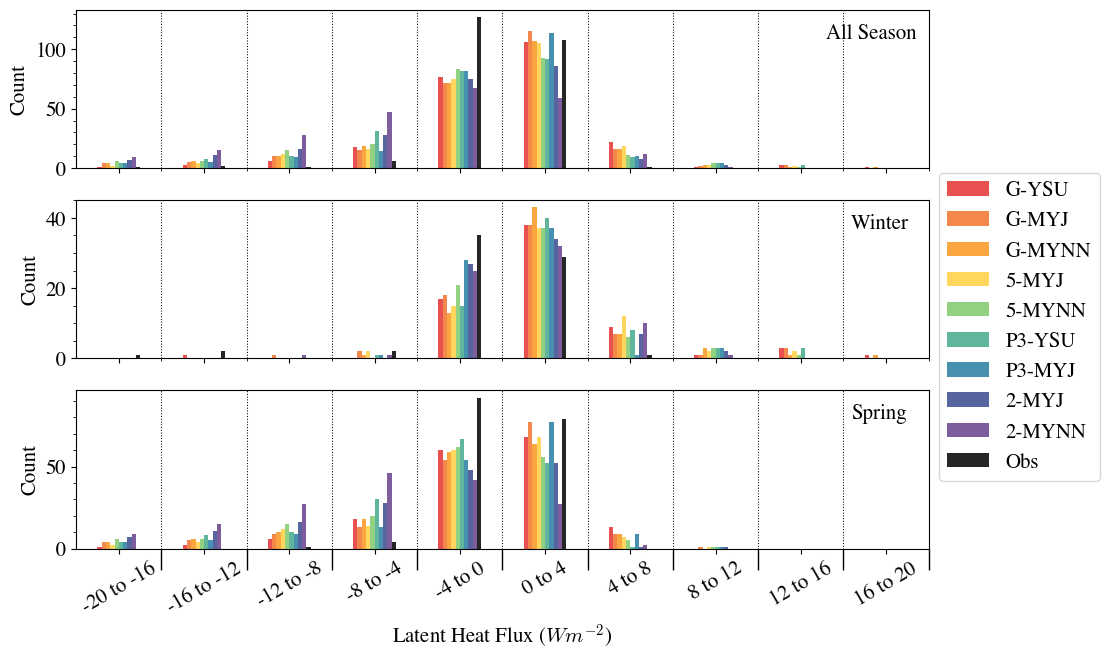
\includegraphics[width=1\linewidth]{figures/chapter3/WRF_LHF_Histo.png}
    \caption[Polar WRF simulated latent heat flux histograms.]{Latent heat flux for the entire observational period (top), winter (middle), and spring (bottom) for each of the Polar WRF runs. Measurements are shown in black and each model simulation is a different color, identified by the abbreviations defined in Table \ref{tab:schemes}.}
    \label{fig:wrf_hlf}
\end{figure}

\begin{figure}[h]
    \centering
    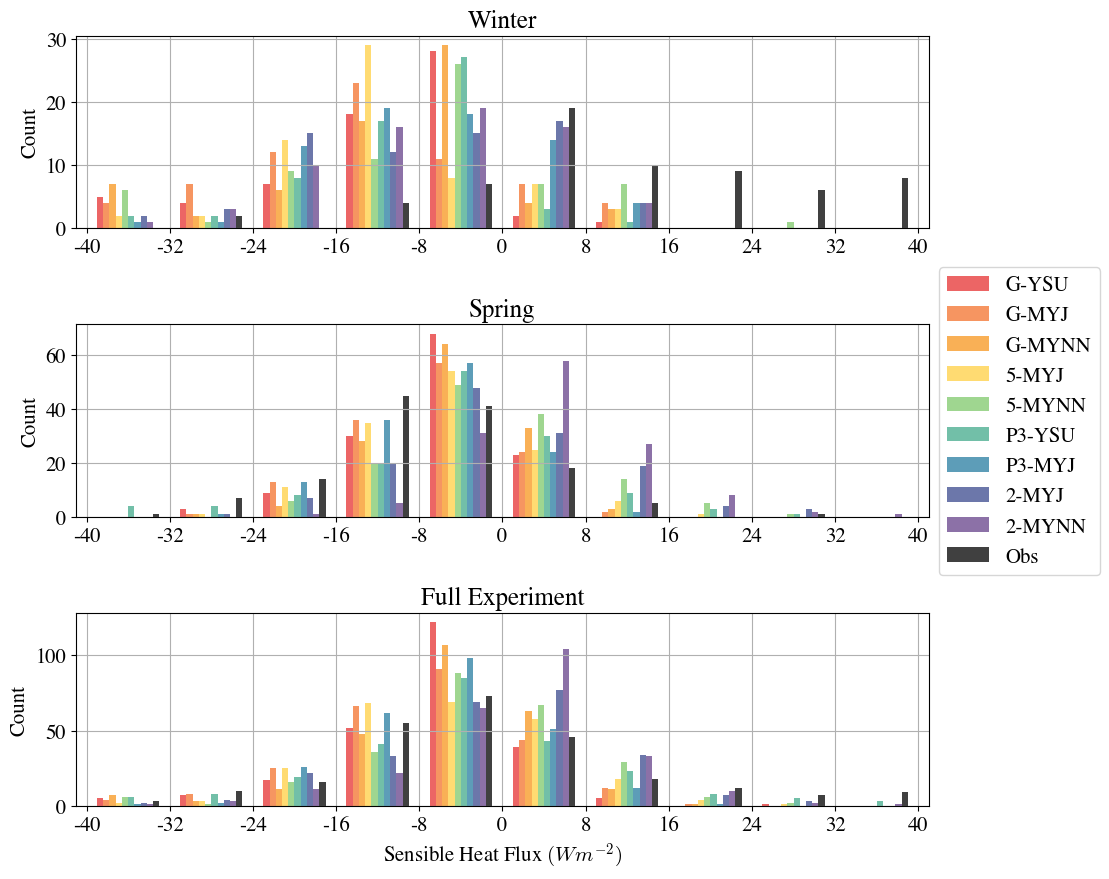
\includegraphics[width=1\linewidth]{figures/chapter3/WRF_SHF_Histo.png}
    \caption[Polar WRF simulated sensible heat flux histograms.]{Sensible heat flux for the entire observational period (top), winter (middle), and spring (bottom) for each of the Polar WRF runs. Measurements are shown in black and each model simulation is a different color, identified by the abbreviations defined in Table \ref{tab:schemes}.}
    \label{fig:wrf_shf}
\end{figure}

Figures \ref{fig:wrf_hlf} and \ref{fig:wrf_shf} show the latent and sensible heat flux, respectively. The magnitudes of the latent heat flux measurements were close to zero throughout the entire period \citep{walden:2017}, but modeled values ranged from -20 to +20 $Wm^{-2}$. All model simulations produced inaccurate latent heat flux values as they all calculated a much larger range of values about 0 $Wm^{-2}$. This indicates more phase change was occurring in the simulations than was actually observed. The wide range of values in the model compared to the measurements indicates this model is producing more deposition/sublimation and freezing/melting than is actually occurring. 

In the spring, the calculations of the latent heat flux were similar in all the model simulations but varied more largely than the measurements. The measurements peaked at zero with limited spread, slightly favoring the negative values (melting, sublimation, or evaporation). All the model simulations, however, overestimated the amount of melting/sublimation/evaporation that was occurring by overestimating the amount of negative latent heat flux. 

In the winter, the calculation of sensible heat flux is incorrect in all of the model simulations and is most influenced by the PBL scheme. The YSU PBL scheme shows a peak between 0 and 10 $Wm^{-2}$, but a smaller spread than the measurements, indicating that this scheme is underestimating the near-surface lapse rate. The MYJ PBL scheme, however, has the opposite problem. The spread is too large, indicating that the fluxes between the surface and atmosphere are too large, resulting from a larger lapse rate. Neither scheme accurately represents the distribution of the measurements, which is less steep at positive flux values. The runs using the MYNN PBL scheme had the lowest flux bias values.

The sensible heat fluxes in spring peak just below 0 $Wm^{-2}$ in the measurements, but were slightly positive in the model simulations, indicating that the model predicted the atmosphere was warmer than the surface and flux was going into the surface. The MYJ PBL scheme predicted a small secondary peak slightly negative that was also captured in the measurements, but the shape, value, and magnitude of this peak were incorrectly simulated by the model. The sensible heat flux calculations by the MYJ PBL scheme compare well to the measurements; the MYNN PBL scheme performs worse. The measurements and the 2-MYNN simulation both show a large spread with slightly more negative sensible heat fluxes than the other simulations. This indicates that there is a greater flux out of the surface in the 2-MYNN scheme and in the measurements, as the surface temperature is less than the air temperature.

\subsection{Case Studies}
\citet{cohen:2015} described synoptic events (major and minor storms) during N-ICE that caused short-term changes in the local weather conditions. A winter and a spring case study are described below to determine how well the WRF simulations were able to capture these short-term events.

\subsubsection{Case 1 - A Winter Cold Frontal Passage, 5 February 2015}
\begin{figure}[p]
    \centering \hspace*{-0.75cm}
    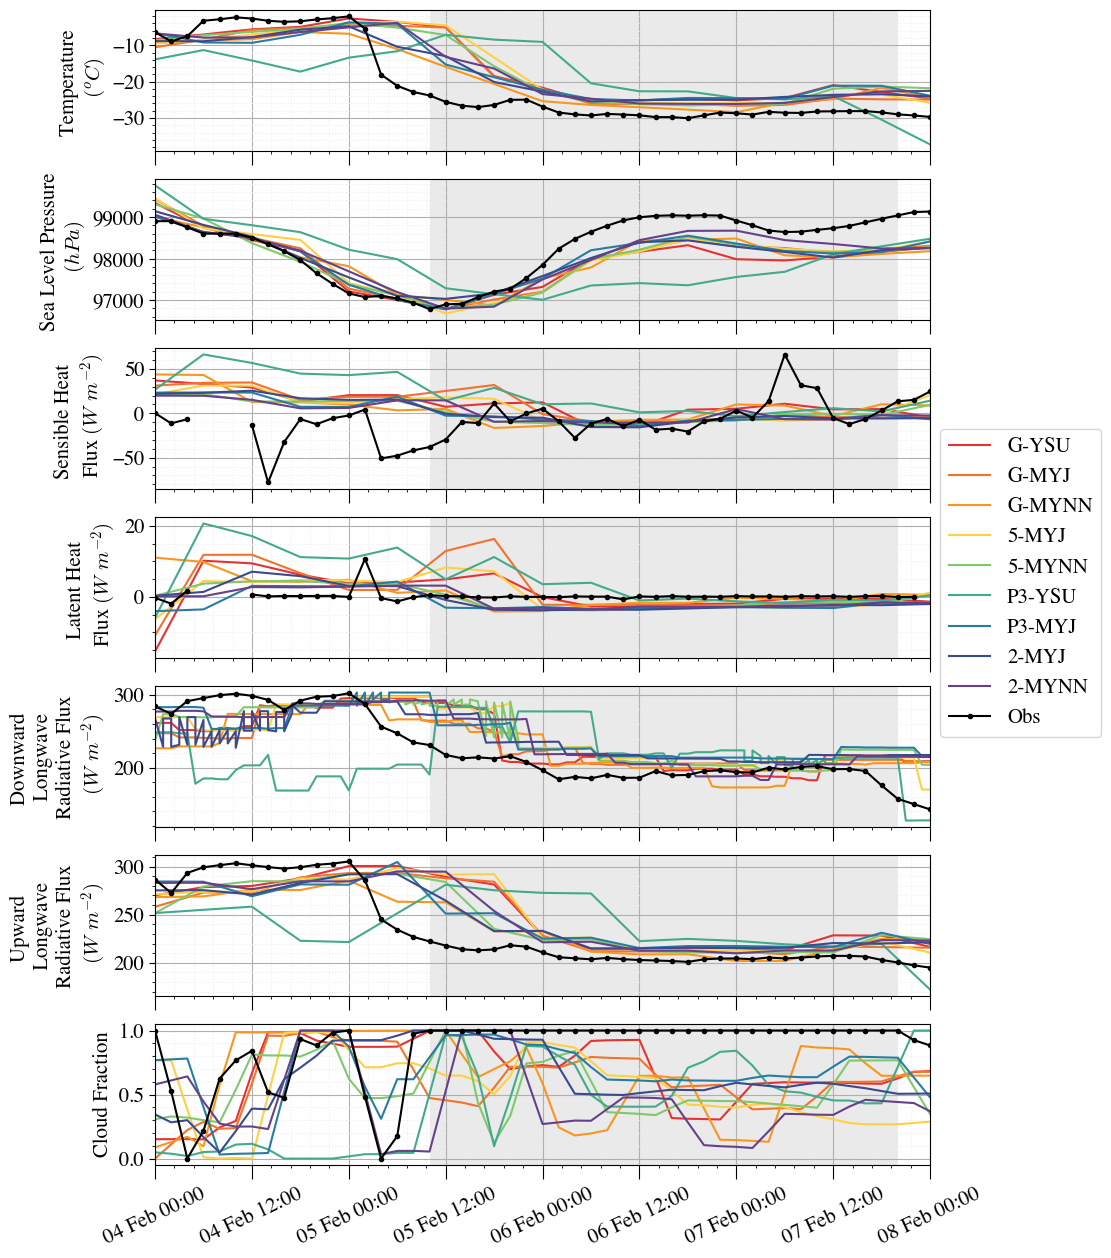
\includegraphics[width=1.1\linewidth]{figures/chapter3/wrf_case1.png}
    \caption[Polar WRF Case 1 - Winter cold front (5 Feb 2015) time series]{6-hourly values of WRF modeled output (rainbow, acronyms in legend defined in Table \ref{tab:schemes}) and observations (black) for temperature, sea level pressure, sensible heat flux, latent heat flux, downward longwave flux, upward longwave flux, and cloud fraction during the cold-frontal passage from 4 Feb to 8 Feb 2015.}
    \label{fig:wrf_case1}
\end{figure}

A cold front passed through the ship location just after midnight on 5 February, bringing a temperature drop of approximately 25$^{\circ}C$. \citet{cohen:2017} indicated this was the second major storm that passed over the ship during the observation period. The model simulations do not accurately capture the timing or magnitude of the cold front. Prior to the frontal passage, observed temperatures were warmer than those forecasted by WRF (top panel, Figure \ref{fig:wrf_case1}). Additionally, after the front passes, the modeled temperature is, at times, around 10$^{\circ}C$ higher than the measured temperature. This can also be seen in both components of the longwave flux (Figure \ref{fig:wrf_case1}, 5th and 6th panel from the top). P3-YSU performed particularly poorly during this period; this run had the lowest pre-frontal temperature and took the longest for temperatures to fall after the passage of the front.

A possible explanation for the P3-YSU scheme performing so poorly with temperature and longwave flux is the lack of cloud cover before the front. This scheme consistently produced close to zero cloud cover ahead of the front. While the observations did not see complete cloud cover until just after the front passage on 5 February at 12:00 (indicated by gray shading in Figure \ref{fig:wrf_case1}), the ship still experienced some cloud cover, at times approaching 100$\%$ over the six-hour averaging period. The P3-YSU scheme did not produce any cloud cover ahead of the front, and cloud cover reduced quickly after the frontal passage, which was not seen in the measurements. 

During the first half of this case, the sensible heat flux values in the measurements were negative, indicating that the surface was warmer than the atmosphere. The model, however, produced positive sensible heat flux values during this time for all combinations of PBL and CM schemes. Latent heat flux is also largely positive in the model simulations during this time, while the observations consistently observed latent heat flux values near zero. 

The two simulations using the Morrison 2-Moment CM scheme performed the best in this case. These simulations consistently had cloud cover that compared well to the measurements during the first half of this case. They also performed the best for each of the other variables shown in Figure \ref{fig:wrf_case1} throughout the entire case study regardless of the reduction in cloud fraction each experienced during the second half of the case. The ability of the model to simulate the fluxes, in this case, seems to depend on how well the simulations can reproduce the cloud fraction.

\subsubsection{Case 2 - A Spring Clear-Sky Day, 23 May 2015}
\begin{figure}[p!]
    \centering \hspace*{-0.75cm}
    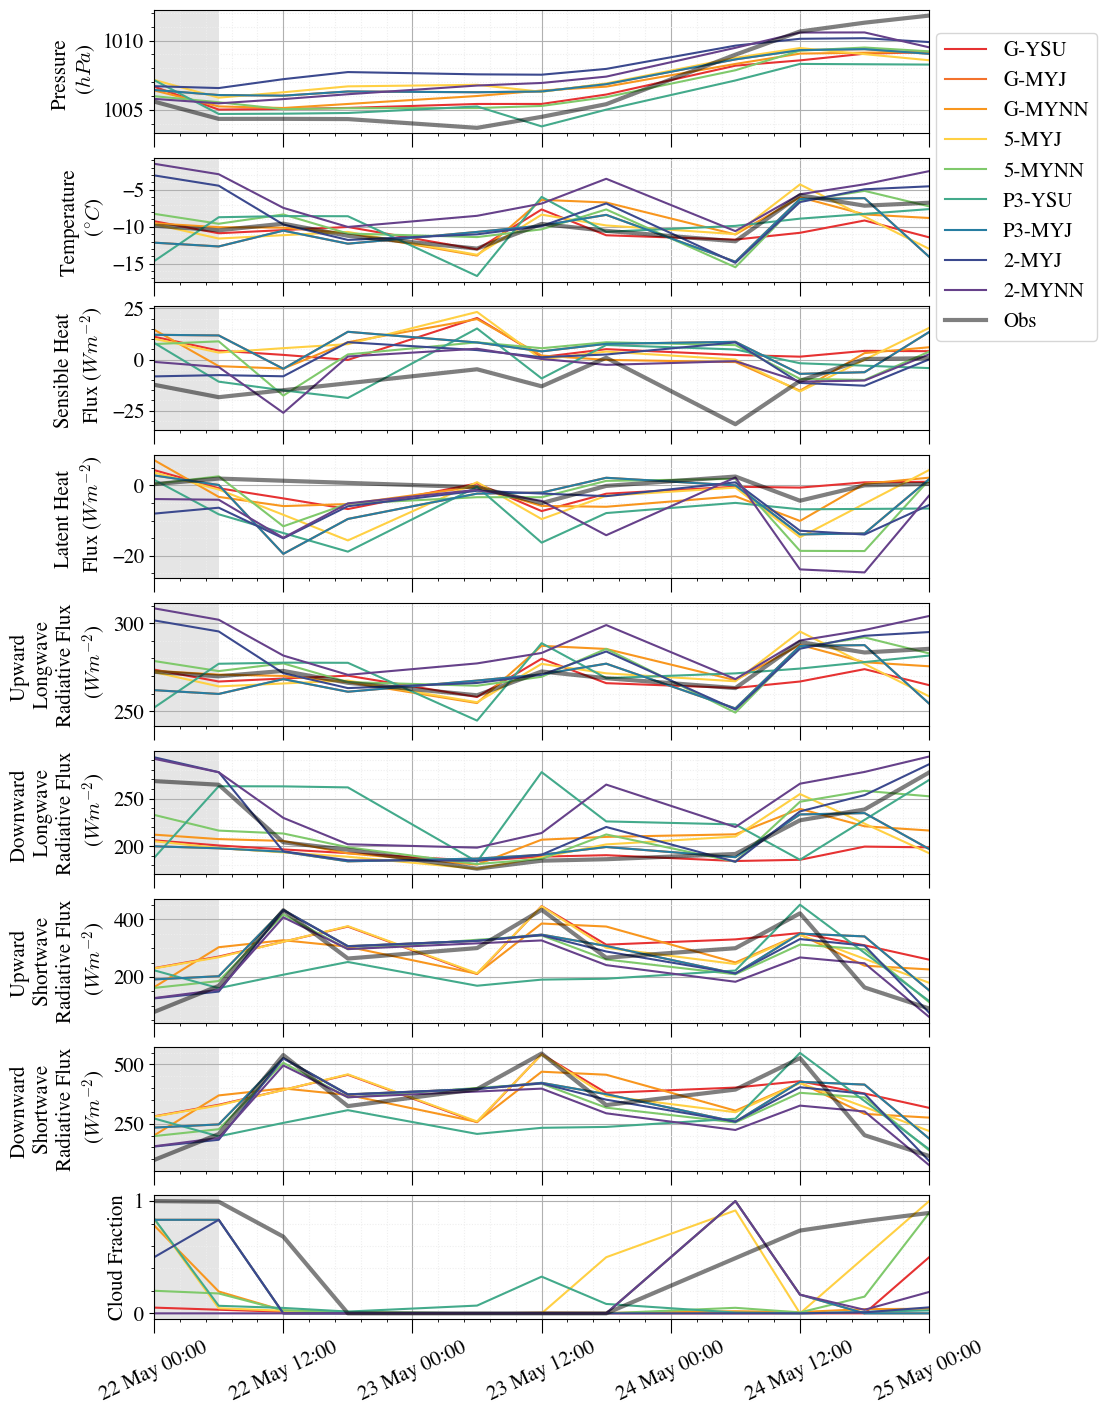
\includegraphics[width=1.1\linewidth]{figures/chapter3/wrf_case2.png}
    \caption[Polar WRF Case 3 - Spring clear-sky (23 May 2015) time series]{6-hourly values for WRF modeled output (6-hourly, rainbow, acronyms in legend defined in Table \ref{tab:schemes}) and observations (6-hourly, black) for temperature, sea level pressure, sensible heat flux, latent heat flux, downward longwave flux, upward longwave flux, downward shortwave flux, upward shortwave flux, and cloud fraction during the spring clear-sky period from 22 May to 25 May 2015.}
    \label{fig:wrf_case2}
\end{figure}

Clouds occurred nearly continuously during the spring at N-ICE, however, the only 24-hour period of clear skies occurred on 23 May. Observations and WRF output variables during this time period can be seen in Figure \ref{fig:wrf_case2}. In contrast to the winter cold-front case, the Morrison 2-Moment schemes seem to be performing worse than the other schemes during this case study. Temperatures in the simulations using the Morrison 2-Moment scheme were higher than the other simulations, with temperatures almost 20 $^{\circ} C$ above the observations during the 10 hours of clouds seen on the 22nd prior to the start of the clear-sky period. Many of the schemes simulated the clear-sky period correctly with the exception of the P3-YSU model run, which produced some clouds mid-day on the 23rd. This run also had difficulties with the downward longwave throughout this period, with large swings between 190 and 250 $W~m^{-2}$. 

Model runs using the Goddard CM scheme performed the best during the clear-sky period, with latent heat fluxes close to zero and longwave radiative fluxes closest to the measurements. These schemes also had the most accurate surface temperatures.

\section{Conclusions}
In this study, Polar WRF was used to simulate surface fluxes over first-year sea ice from January to June 2015. Model results were compared to observations taken during the N-ICE field campaign. A collection of CM and PBL schemes were selected based on a literature survey of previous modeling studies both in the Arctic and elsewhere. 

The schemes using the Morrison 2-Moment CM had the lowest biases in latent heat flux in the winter overall and performed best in the winter cold front case study. However, the overall temperature biases from these schemes were the largest in the winter, indicating that these schemes perform best under conditions like those seen in the winter case study, when the model did accurately forecast temperatures. The P3 CM scheme performed the worst in the winter, with the highest biases in both longwave flux, sensible heat flux, and temperature. 

In the spring, latent and sensible heat fluxes produced by simulations using the Morrison 2-Moment scheme had the largest biases. Additionally, schemes using the MYNN PBL scheme had larger biases than simulations with other PBL schemes, generally producing a larger sensible heat flux than was observed. This indicates that, particularly in the spring, the MYNN PBL scheme is not producing the correct near-surface temperature structure. 

The time of year and the near-surface atmospheric temperature structure are important to consider when selecting CM and PBL schemes. In the winter when surface inversions are more likely to be present, the MYNN scheme produces the most accurate sensible heat flux estimations. However, the MYJ scheme appears to perform best for the latent heat flux and temperature. In the spring, when mixed-phase clouds are more common and the surface is starting to melt, the MYJ scheme still excels at estimating the latent heat flux and has some of the lowest biases. 

The next chapter will describe the cloud conditions at N-ICE to give perspective into the conditions the model is trying to simulate. Cloud radiative forcing from the model is also calculated and explored for the 2-MYNN and G-YSU model simulations, as these had some of the lowest overall biases in winter and spring/summer, respectively. Chapter 5 looks at the equations used to calculate the sensible and latent heat fluxes and examines them independently of the model to determine if these equations could be at fault for some of the inaccuracies in the model output. The chapter 5 also explores alternative ways of calculating the stability equations and the fluxes themselves in an attempt to improve modeled fluxes. Chapter 6 will conduct sensitivity studies to determine if improvements can be made to the model. To conclude, Chapter 7 uses lessons learned in the previous chapters to make recommendations for changes in Polar WRF over first-year sea ice. 